\chapter{Closed-loop Model Simulation/Testing}
Model checking is performed on abstract models of the system and/or its environment, which means that if the model checker returns a counter-example, it will be an abstract execution. An abstract execution may correspond to multiple concrete executions and the ambiguity has to be resolved. Closed-loop simulation/testing are performed on more refined model or the actual system thus can complement model checking in terms of resolving ambiguities. In this chapter we first demonstrate the tool we developed to translate a verified UPPAAL model to Stateflow charts. Then we demonstrate two examples that cannot be explicitly modeled using abstract semantics.

\begin{itemize}
	\item What are the limitations of model checking?
    \item How can simulation complement that?
\end{itemize}
\section{UPP2SF Automated Translation}
Consider an UPPAAL model with automata $P_1,...,P_n$. The UPP2SF translation procedure would produce a two-level Stateflow chart as in \figref{chart}, with parallel states $P_1,...,P_n$ (referred to as the \textit{parent} states) derived from the automata, parallel states $Gc\_{x_1},..., Gc\_{x_m}$ (referred to as \textit{clock states}) that model all global clocks $x_1,...,x_m$ from the UPPAAL model, and the state $Eng$ that is used as the chart's control execution engine.
In addition, the chart has predefined global data variables (and constants) with appropriate variable ranges and initial values obtained from the UPPAAL model. 
Since all automata in UPPAAL are simultaneously active, the obtained Stateflow chart is a collection of parallel states with unique execution orders. Also, in every UPPAAL automaton exactly one location is active at a time. Thus, each of the parent states is a collection of exclusive states, extracted from locations in the UPPAAL automaton.
\begin{figure} [!t]
\center
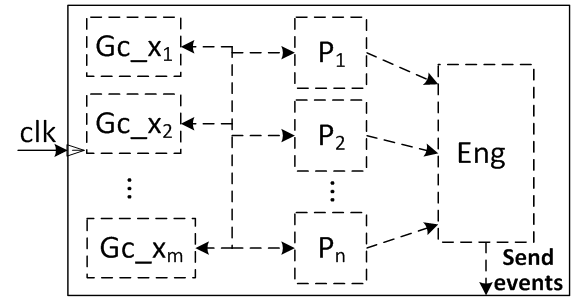
\includegraphics[width=0.6\textwidth]{figs/chart_GlobalClocks_rev1.png} 
\caption{Structure of Stateflow charts derived by UPP2SF. Parent states $P_1,...,P_n$ are derived from automata, while the \textit{clock} states $Gc\_{x_1},..., Gc\_{x_m}$ model all global clocks $x_1,...,x_m$ from the UPPAAL model. The state $Eng$ is used to control execution of the chart.}
\label{fig:chart}
\end{figure}

The UPPAAL model of the DDD pacemaker model in \figref{PMdesign} is translated into Stateflow chart presented in \figref{PM_sf} using the UPP2SF tool.
\begin{figure*} [!t]
\center
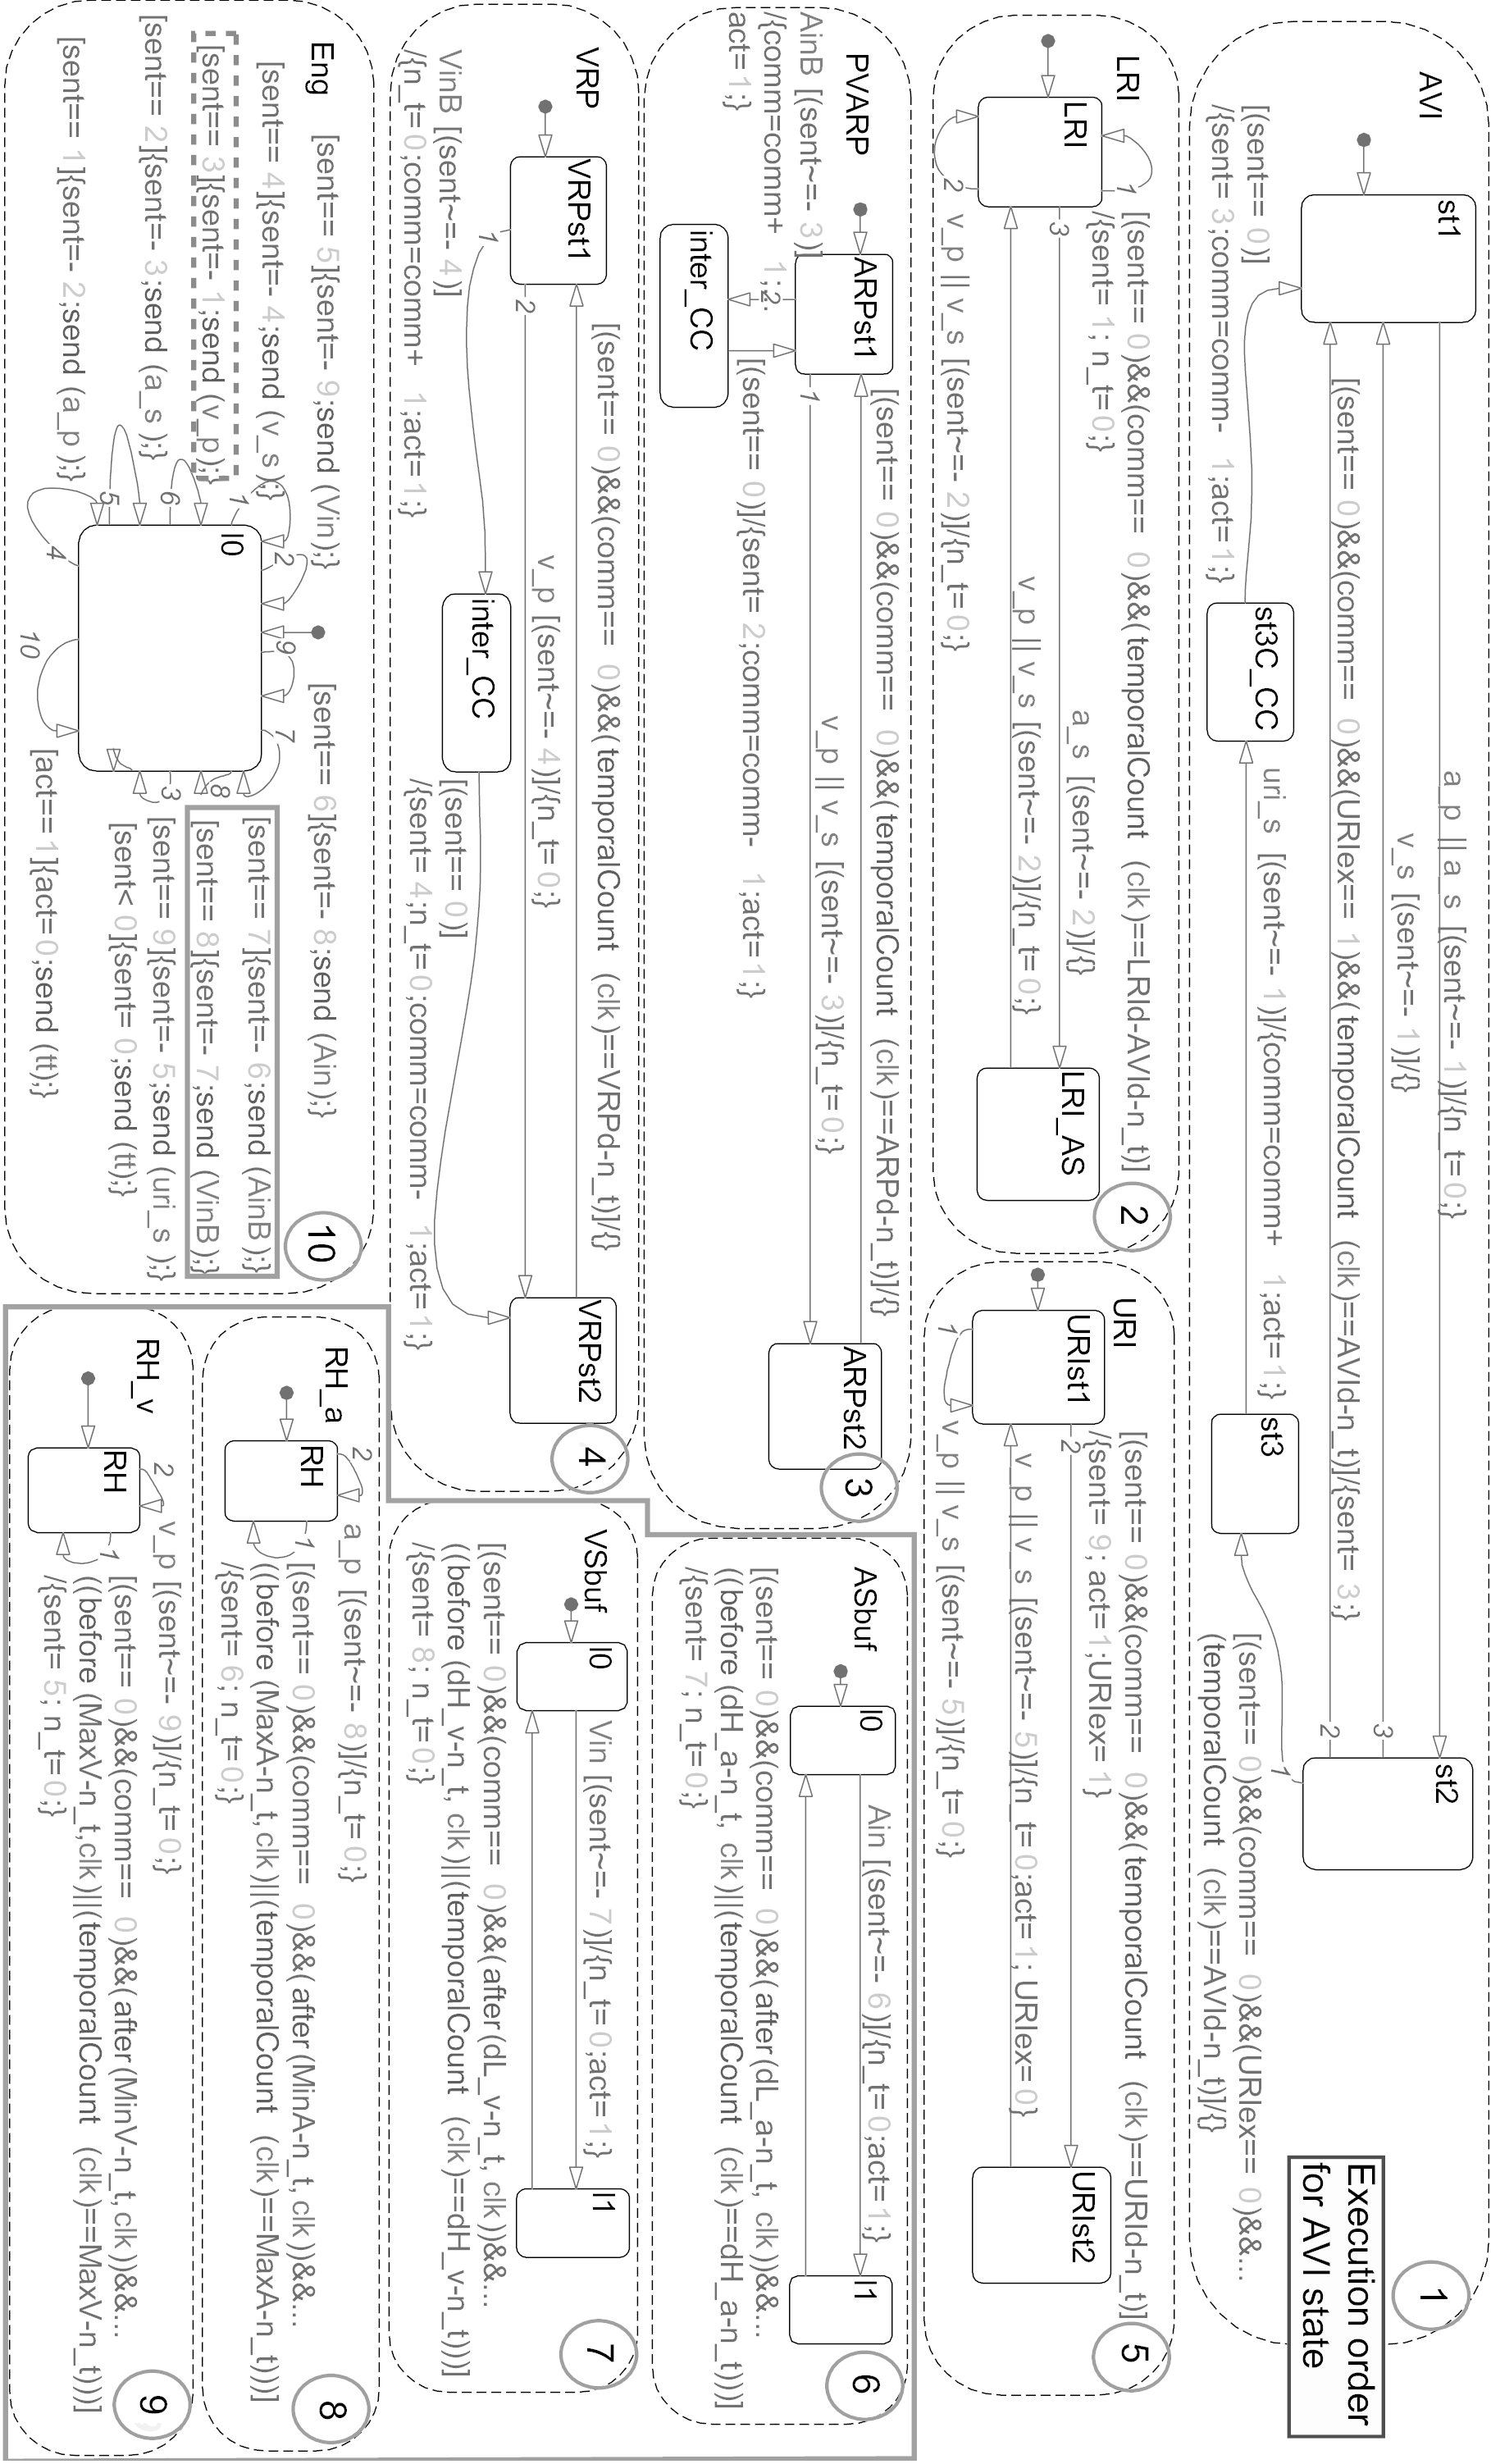
\includegraphics[width=1.00\textwidth]{figs/PM_SF_buffer_newC1.png} 
\caption{Pacemaker Stateflow chart extracted using UPP2SF from the UPPAAL model in~\figref{PMuppaal}; the heart and buffer models are highlighted.} 
\label{fig:PM_sf}
\end{figure*}

We generated C code from the pacemaker Stateflow chart using the Simulink Coder. The code structure is shown in \figref{pm_code}.
The code was generated for the general embedded real-time target and as a result we obtained the main procedure, \texttt{rt\_OneStep}, which processes the three input events, $VinB$, $AinB$ and $clk$. To ensure that the model semantics is preserved (modulo the execution time), $clk$ input events should be created every 1ms, followed by the procedure's activation. This makes it suitable for implementation on top of a real-time operating system (RTOS).

\begin{figure*} [!t]
\center
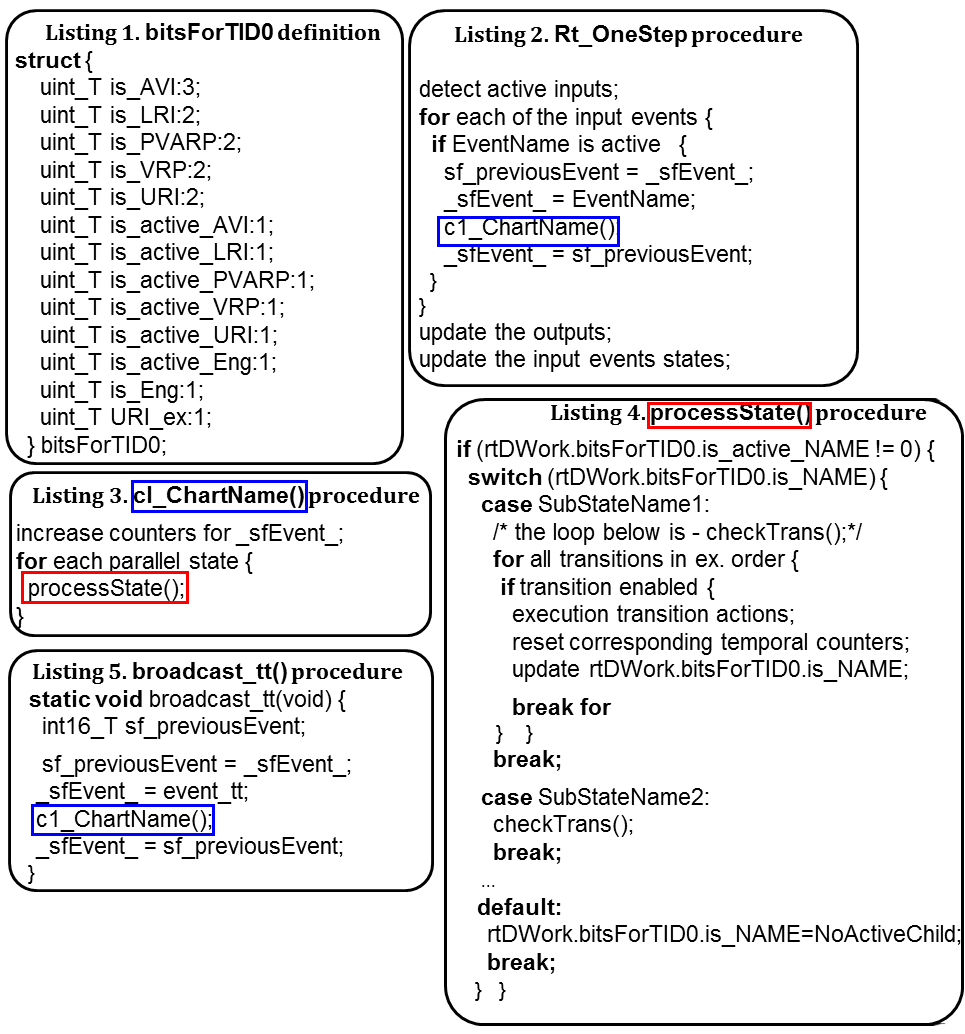
\includegraphics[width=0.77\textwidth]{figs/CodeListingFinal.png}
\caption{Structure of the pacemaker code obtained from the Stateflow chart shown in \figref{PM_sf}.}
\label{fig:pm_code}
\end{figure*}


The pacemaker code generated by the Simulink RTWEC was executed on nanoRK~\cite{nanork}, a fixed-priority preemptive RTOS that runs on a variety of resource constrained platforms. We tested the implementation on the TI MSP-EXP430F5438 Experimenter Board interfaced with a signal generator that provides inputs for the pacemaker code (\figref{setup}). More details regarding UPP2SF translation can be found in \cite{TECS}.

\begin{figure} [!t]
\center
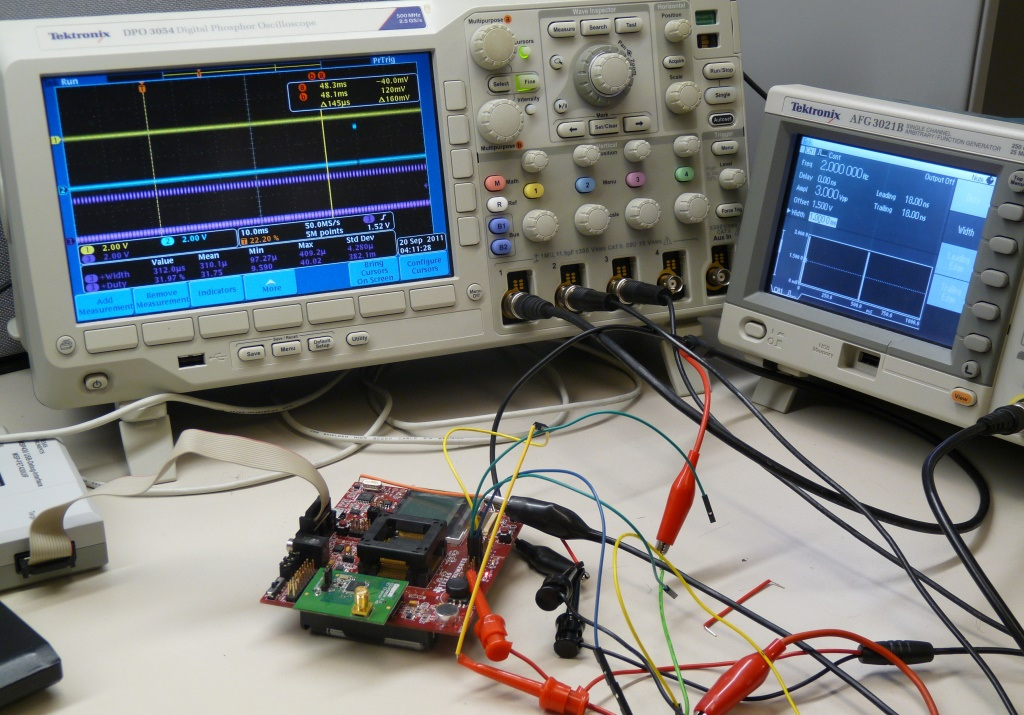
\includegraphics[width=0.5\textwidth]{figs/HW_setup1.png}
\caption{Hardware setup with MSP430F5438 experimenters board.}
\label{fig:setup}
\end{figure}

\section{Crosstalk}
Oversensing is a general term for inappropriate sensing caused by noise or far-field signals. It's very common among pacemaker malfunctions and it may result in failure to pace, competitive pacing and inappropriate therapy. Crosstalk is a special case for oversensing which occurs when the pacemaker stimulus in one chamber is sensed in the other chamber. It happens when two leads are close to each other or pacing signal in the other chamber is too strong. It is common that the ventricular lead is placed in the right ventricle outflow tract, which is close to the atrium. \figref{crosstalk}(a) shows simulated EGMs from a patient with bradycardia and complete heart block. During atrial pacing (AP), the pacing signal is sensed by the ventricular lead 53 ms after the AP. (Marker 1) It is treated as ventricular sense (VS) signal and thus inhibit the subsequent ventricular pacing (VP). This is indicated by no QRS-wave in the ECG channel. (Marker 2) For a patient with complete heart block this will cause dangerous ventricular asystole.  

Increasing the sensing threshold of the ventricular channel can prevent false sensing. In \figref{crosstalk}(b), the small signals in ventricular EGM are ignored and ventricular pacing are successfully delivered. 
\begin{figure*}[!t]
\center
\vspace{-10pt}
		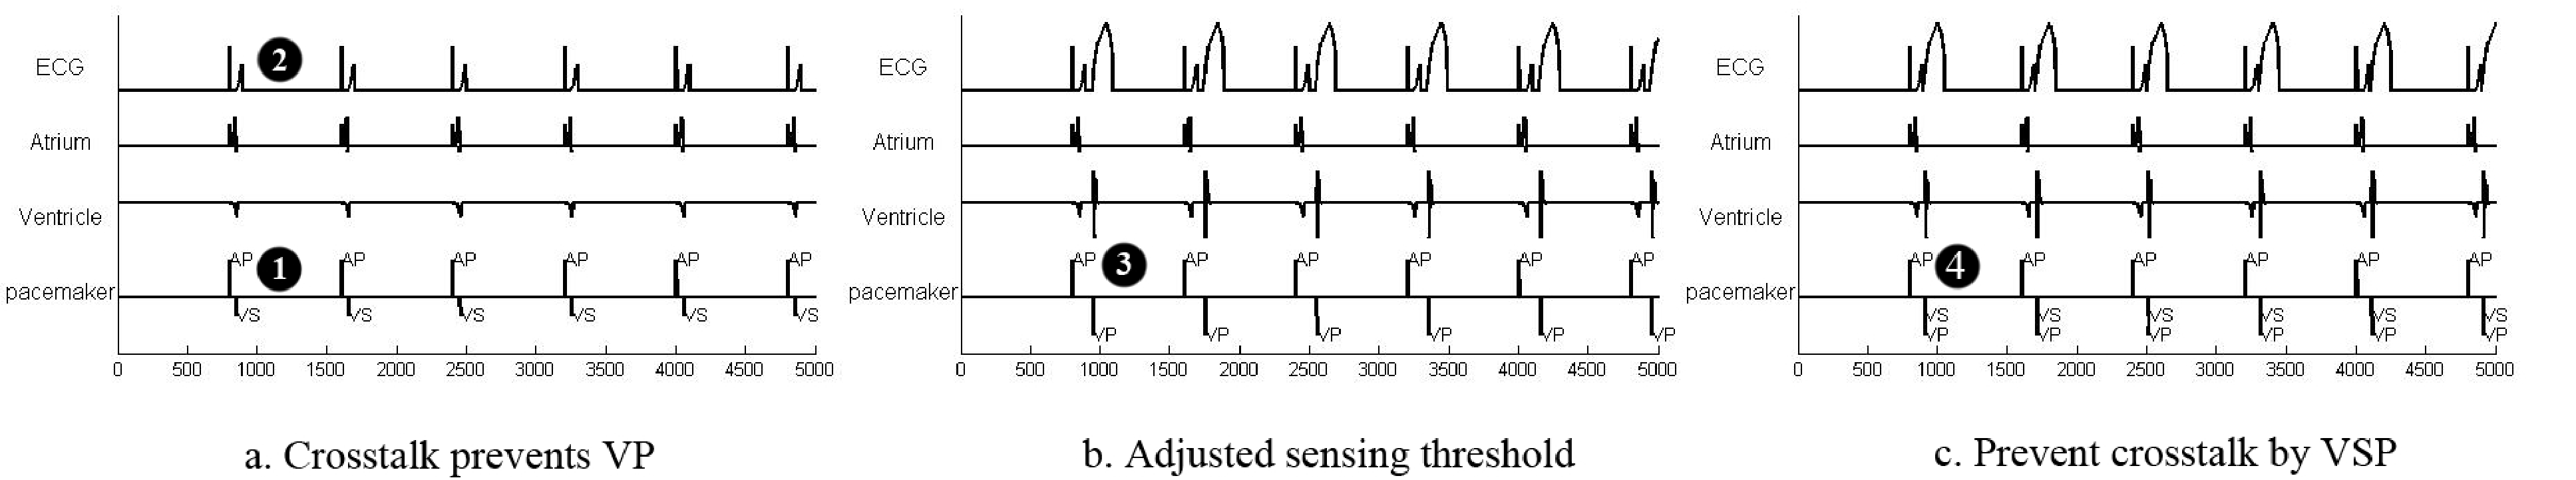
\includegraphics[width=\textwidth]{figs/crosstalk_all.pdf}
\vspace{-20pt}
\caption{Crosstalk between pacemaker leads with high sensitivity in the ventricle, adjusted sensitivity and ventricular safety pacing}
\label{fig:crosstalk}
\vspace{-15pt}
\end{figure*}
\section{Lead Displacement}
Lead displacement affects many patients and can result in inappropriate or ineffective therapy. \figref{dislodge_norm} shows the simulation result for the pacemaker function when the leads are in their designated location. From the figure we can observe: 1) Each P-wave is initialized by an Atrial Pace signal. 2) Each QRS complex is initiated by a ventricular pacing signal. 3) The interval between AP and VP is 150 ms, which matches the programed AVI period.

One common case for lead dislodge is shown in \figref{race_cond}, where the atrial lead has fallen into the right ventricle outflow tract. In this case the atrial lead senses from the ventricle rather than atrium and atrial pacing will initiate a ventricular event. \figref{dislodge} shows the simulated EGMs in this case. The figure reveals several facts: 1) No P wave is sensed or tracked (Marker 1). 2) Atrial Pace initiates an abnormal, wide QRS which is then sensed by the ventricle lead (Marker 2). 3) Intermittent appearance of VP on QRS 110 ms after the AP. The ventricular lead can receive signal from: 1) pacing signal sent from the atrial lead, 2) the intrinsic A-V conduction path. The two path are shown in \figref{race_cond} and form a timing race condition. When the signal from the atrial lead arrives the ventricular lead first, it will trigger VS. If the intrinsic signal arrives the ventricular lead during the VSP sensing window (defined in previous section), it will trigger VSP. Although the pacing is 'safe' because the pacing is early enough to avoid the vulnerable refractory period, the damage caused by pacing on depolarized tissue is currently a matter of much investigation.     


%%\chapter{Certification}
%%\begin{itemize}
%%          	\item What is the current practice for medical device certification? What are the limitations?
%%          	\item Can model-based closed-loop verification provide more safety guarantee to complement current practice? By how much?
%%          \end{itemize}
%%          
%%\section{Current Practice}
%%%In United States, medical devices have to be approved by FDA to be released into the market. 
%%According to their potential risks the devices are categorized into 3 classes, Class I, Class II and Class III, corresponding to low-risk, medium-risk and high-risk devices \cite{class}. Life-sustaining devices like implantable pacemakers are classified as Class III and in general are subject to the most strict regulations.
%%
%%There are two processes that a medical device can enter the market in U.S.: the Premarket Notification, also known as 510(k) \cite{510k}, and the Pre-Market Approval (PMA) \cite{PMA}. In a 510(k) submission the device manufacturers are only required to provide evidence that the device is \emph{substantial equivalent} to a \emph{predicate device}, which has been approved for the market. Therefore, the 510(k) submission does not directly require clinical evidence for the safety and effectiveness of the device, thus is suitable for mostly low-risk devices like Class I and Class II devices.  The Pre-Market Approval (PMA) submission is a more stringent regulatory process in which direct clinical evidence is required to prove the safety and effectiveness of the device. However, not all Class III devices are subject to PMA submission. If a Class III device clears the 510(k) process and FDA has not requested PMA for that device, the device is still cleared for market release. A study shows that for Class III devices which PMA has been requested, the levels of evidence varies. Only 40\% of the PMA submissions are supported by controlled clinical trials, which provide the most rigorous clinical evidence \cite{cert_prob}. The lack of quality evidence is usually due to the high cost of the controlled clinical trials.
%%\section{Evidence from Model-based Design}
%%%\cite{pancreas}
%%Model-based verification provides a low-cost solution to provide reasonable evidence for the safety and effectiveness of the devices. The open questions are:
%%
%%\begin{itemize}
%%	\item How valid are the models?
%%	\item How much confidence can they provide?
%%\end{itemize}
